\chapter{Expanding Endomorphisms}\label{c15}

We\pageoriginale will be concerned for the remainder of these lectures with
constructing exotic examples of certain natural structures. We start
this program by constructing in this lecture exotic examples of one of
the simplest types of dynamical systems; namely, of expanding
endomorphisms.

\begin{defi}\label{c15:defi15.1}
  Let $M$ be a closed smooth manifold. A self-map $f: M \to M$ is said
  to be an expanding endomorphism provided $M$ supports a Riemannian
  metric such that $|df (v)|> |v|$ for every non-zero vector $v$
  tangent to $M$.
\end{defi}

\begin{qus}\label{c15:qus15.2}
  What closed smooth manifolds support expanding endomorphisms?
\end{qus}

The question is answered up to topological classification as follows
by results due to Shub \cite{89}, Franks \cite{52} and Gromov
\cite{53}. 

\begin{thm}\label{c15:thm15.3}
  If a closed smooth manifold $M$ supports an expanding endomorphism,
  then $M$ is homeomorphic to an infranilmanifold.
\end{thm}

Recall that infranilmanifolds were definde in \ref{c1:sec1.4}. Shub
showed that the universal cover $\tilde{M}$ of $M$ is diffeomorphic to
$\mathbb{R}^m$ where $m= \dim M$. Then Franks showed that $\pi_1 M$ has
polynomial growth and that $M$ is homeomorphic to an infranilmanifold
provided $\pi_1 M$ is virtually solvable. Gromov completed the proof
of \ref{c15:thm15.3} by showing that a group of polynomial growth must
be virtually nilpotent. Gromov's result was motivated by Hirsch's
paper \cite{60} where it is shown that the solution to Hilbert's fifth
problem is related to \ref{c15:thm15.3}. Hirsch also implicily poised
Question \ref{c15:qus15.2} in his Remark 1; i.e., whether the word
``homeomorphism'' can be replaced by ``diffeomorphism'' in 15.3. But
Farrell and Jones showed in \cite{35} that this is not the case;
namely, they proved the following result.

\begin{thm}\label{c15:thm15.4}
  Let $T^n$ be the $n$-torus $(n > 4)$ and $\Sigma^n$ an arbitrary
  homotopy sphere, then the connected sum $T^n\# \Sigma^n$ admits an
  expanding endomorphism.
\end{thm}

When $\Sigma^n$ is not the standard sphere, Wall [96 \S 15A] showed
that $T^n \# \Sigma^n$ is not diffeomorphic to $T^n$. This fact
combined with the classical rigidity results of Bieberbach
\cite{6}\pageoriginale and Malcev \cite{70} yields that $T^n \#
\Sigma^n$ is \textit{not} diffeomorphic to any infranilmanifold. More
details of this argument will be given in lecture \ref{c16}. The
remainder of this lecture is devoted to constructing the expanding
endomorphism $f: T^n \# \Sigma^n \to T^n \# \Sigma^n$ posited in
\ref{c15:thm15.4}.

Let $\theta_n$ denote the Kervaire-Milnor group of homotopy
$n$-spheres $(n \geq 5)$. We note that $\theta_n = \mathcal{S}^s
(S^n)$ as sets and the abelian grouup structure on $\theta_n$ is given
by the connected sum operation of oriented manifolds;
cf. \cite{65}. Kervaire and Milnor prove that $\theta_n$ is a finite
group and that it is a non-trivial group for infinitely many $n$. They
also calculate its order $|\theta_n|$ for small values of $n$. this
calculation is given by the following table:

\medskip
\begin{tabular}{|c|ccccccccccc|}
\hline
$n$ & 5 & 6 & 7 & 8 & 9 & 10 &  11& 12 & 13 & 14 & 15\\
\hline
$\mid \theta_n \mid$ & 1 & 1 & 28 & 2 & 8 & 6 & 992 & 1 & 3 & 2 &
13.256\\
\hline
\end{tabular}
\medskip

Let $\mathcal{S}$ denote the order of $[\Sigma^n]$ in $\theta_n$ and
set $t= ms + 1$ where $m$ is a \text{large} positive integer. Let
$\ob{f}: T^n \to T^n$ be multiplication by $t$. (Recall $T^n$ is an
abelian group.) It is an expanding endomorphism. The exotic expanding
endomorphism $f$ is topologically conjugate to $\ob{f}$ and is
constructed as the composite of the 4 maps illustrated in the diagram
below; i.e., $f= P \circ E \circ D \circ F$. (In the illustration, $s=2$.)

\begin{figure}[H]
  \centering{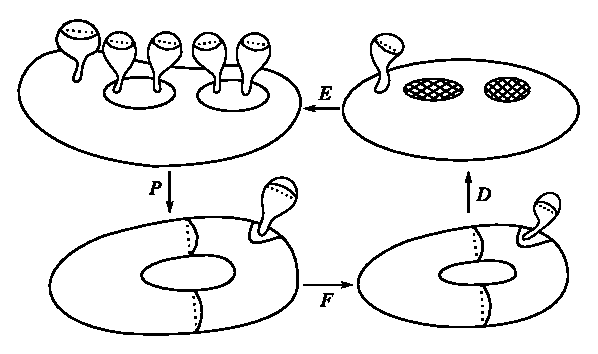
\includegraphics{vol86-figures/fig15.eps}\\
  Figure 15}
\end{figure}

Here\pageoriginale $P$ denotes the covering projection in the standard $t^n$-sheeted
covering space of $T^n \# \Sigma^n$; i.e., the one such that image
$(P_{\#})$ is the subgroup of $\pi_1 (T^n \# \Sigma^n)$ consisting of
all elements divisible by $t^n$. Note that $P$ is a local
isometry. The map $D$ is the diffeomorphism which is uniform dilation
by $t$. It can of course be made as expanding as we want by choosing
$m$ large enough.

The map $E$ is a diffeomorphism with bounded distortion independent of
$m$. It is constructed by carefully grouping the $t^n$-connected
summand of $\Sigma^n$ occuring in its range into sets of $s$-each with
1-summand left over. And then independently ``canceling'' each group
of $s$-summands using the fact that $[\Sigma^n]$ has order $s$. Each
canceled group is illustrated by the shaded disc in the domain of $E$.

Finally, the diffeomorphism $F$ is the identity map outside a closed
$n$-ball $\mathbb{B}^n$ contained in $T^n$. The domain and range of $F$
are both connected sums of $T^n$ with $\Sigma^n$ and $1/t \Sigma^n$,
respectively. Both connected summings occur inside of
$\mathbb{B}^n$. Here, $1/t \Sigma^n$ is the same smooth manifold as
$\Sigma^n$; but its Riemannian metric is dilated by $1/t$. The
diffeomorphism $F$ is constructed ``inside of $\mathbb{B}^n$'' by
using the ``commutator'' $1/t \Phi_t \Phi^{-1}$ illustrated below.
\begin{figure}[H]
  \centering{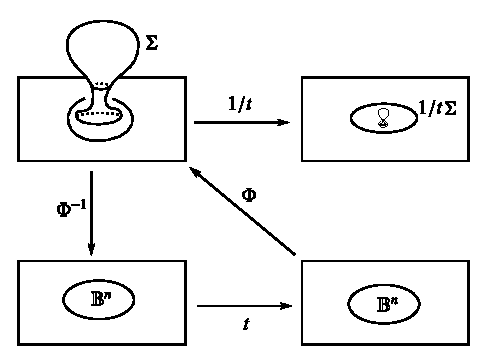
\includegraphics{vol86-figures/fig16.eps}\\
  Figure 16}
\end{figure}

Here\pageoriginale $\Phi: \mathbb{R}^n \to \mathbb{R}^n \# \Sigma^n$
is the diffeomorphism defined as follows. Note first that 
$$
\mathbb{R}^n \# \Sigma^n = \mathbb{B}^n \coprod_\phi (\mathbb{R}^n -
\Int \mathbb{B}^n)
$$
where $\phi: S^{n-1} \to S^{n-1}$ is a self-diffeomorphism and the
identification $\sim$ above is given in polar co-ordinates by 
$$
(x, r)\sim (\phi (x), r) ~\text{where}~ r=1.
$$

(We can take $\mathbb{B}^n$ to be the ball of radius 1 centered at the
origin of $\mathbb{R}^n$.) Then $\Phi$ is defined in terms polar
co-ordinates $(x, r)$ where $x \in S^{n-1}$ and $r \in [0, + \infty)$
  by the formula
$$
\Phi(x, r) = 
\begin{cases}
  (x, r) & \text{if}~ r < 1\\
  (\phi (x), r) & \text{if}~ \geq 1.
\end{cases}
$$

It is easily shown that the ``commutator''
$$
y \mapsto 1/t \Phi(t \Phi^{-1} (y))
$$
is the identity map outside of $\mathbb{B}^n$ and also that its
derivative has bounded distortion independent of our choice of
$m$. Consequently, $f$ is an expanding endomorphism of $T^n \#
\Sigma^n$ provided $m$ is chosen to be sufficiently large. 
